\chapter{Digital pathology}
\label{chap:backdp}

\begin{overview}{Overview}
  The goal of this chapter is to provide digital pathology background  and keys to understand our contributions. We will focus our attention on topics relevant to this thesis. 
  
  Section \ref{sec:backdp:whatisdp} introduces and defines medical terms such as \textit{pathology}, defines \acrfirstit{digital pathology} and introduces the notion of \acrfirstit{wsi}. Section \ref{sec:backdp:wsi} presents the journey of a sample from the body to the \acrshort{wsi}, introducing the different sources of variability introduced by the whole conversion process. 
\end{overview}

% analogintelligence.com image dp illustration

\section{What is digital pathology?}
\label{sec:backdp:whatisdp}

Nowadays, medicine and healthcare rely heavily on analysis of human body samples to study and diagnose diseases. The branch of medicine focusing on this analysis is called \textit{pathology} which includes histology-based pathology (\aka histopathology) or cytology-based pathology (\aka cytopathology). Both of these sub-branches involve the study of microscope glass slides containing samples (see Figure \ref{fig:backdp:glassslides}). In the case of histology, these samples are tissue sections cut from a bodily specimen. Cytology, on the other hand, is concerned with samples of free cells or tissue fragments which can be extracted by different techniques. 

\begin{figure}
  \centering
  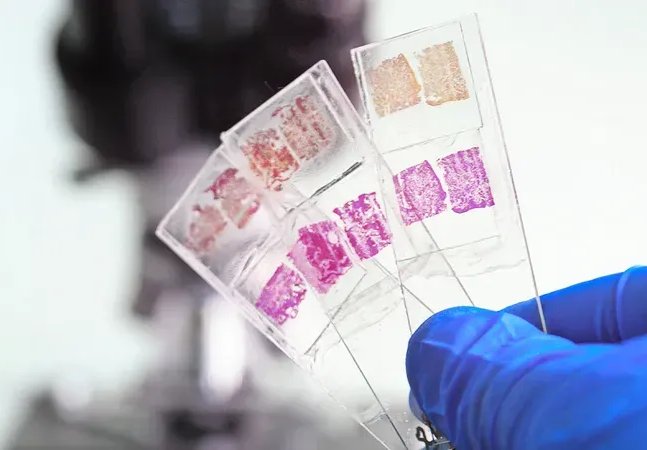
\includegraphics[scale=0.75]{backdp/microscope-slide.png}
  \caption{Microscope slides with tissue samples (image from \parencite{img:glassslides}).}
  \label{fig:backdp:glassslides}
\end{figure}

The trend of digitalization affecting our societies also impacts pathology as, using dedicated scanners, these glass slides can now be digitized into image files called \acrfirstit{wsi}. In this context, \acrfirstit{dp} can be defined as ``\textit{the acquisition, management, sharing and interpretation of pathology information — including slides and data — in a digital environment}'' \parencite{doolan2019whatisdp}. Working with \acrshort{wsi} instead of physical slides has several advantages and drawbacks (see Table 1 in \parencite{jahn2020digital}). Aside from easier sharing and storing of slides, digitization also opens the way for automated analysis sofware to extract relevant information for pathologists.

Whereas automated processing of \acrshort{wsi} is possible, 

\section{Whole-slide images: a journey from the body to the computer}
\label{sec:backdp:wsi}

\parencite{mccann2014automated}

\subsection{Biopsy and smearing}
\subsection{Staining}
\subsection{Scanners}

\section{Professions and typical tasks}
\label{sec:backdp:professionandtasks}

\section{Machine learning}
\label{sec:backdp:ml}

\subsection{Data leakage}
\label{ssec:backdp:dataleakage}

\subsection{Data scarcity}
\label{ssec:backdp:datascarcity}
% and imperfect annotations

\subsection{Transfer learning}
\label{ssec:backdp:tl}

\parencite{van2019strategies}

\section{Visualization and analysis tools}

\subsection{Cytomine}

\subsection{Others}

\section{Digital pathology datasets}
\label{sec:backdp:dataset}


% origin, acknowledgements, subject, organ, staining, statistics


\subsection{Thyroid nodule fine-needle aspiration biopsy}



\subsection{Publicly available}